% !TeX document-id = {a7325568-63cb-46d1-95d6-777a45054e5a}
% !TeX TXS-program:compile = txs:///pdflatex/[--shell-escape]
\documentclass{article}
\usepackage{style}
\begin{document}
\maketitle
\tableofcontents
\section{Introducción}
La red ADALINE(ADAptive LInear NEuron) fue inventada por Bernard Widrow y Marcian Hoff, esta usa un algoritmo de aprendizaje llamado LMS(Least Mean Square). En comparación con el perceptrón, esta usa una función de activacion lineal, solo puede resolver problemas linealmente separables pero esta no es sensible al ruido.
\newpage
\subsection{Modelo}
\begin{figure}[h!]
	\caption{Modelo}
	\centering
	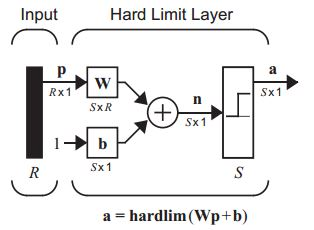
\includegraphics{model}
\end{figure}
\newpage
\section{Diagrama de Flujo}
\begin{figure}[htpb]
	\centering
	\includesvg[width = 400pt, height = 400pt]{diagram}
	\caption{Diagrama de Flujo}
\end{figure}
\newpage
\section{Resultados}
\subsection{Ejemplo 1}
\subsubsection{Datos}
\[p_1=
\begin{bmatrix}
1\\
1
\end{bmatrix}
, t = \begin{bmatrix}
-1\\
-1
\end{bmatrix}
\]

\[p_2=
\begin{bmatrix}
1\\
2
\end{bmatrix}
, t = \begin{bmatrix}
-1\\
-1
\end{bmatrix}
\]

\[p_3=
\begin{bmatrix}
2\\
-1
\end{bmatrix}
, t = \begin{bmatrix}
-1\\
1
\end{bmatrix}
\]

\[p_4=
\begin{bmatrix}
2\\
0
\end{bmatrix}
, t = \begin{bmatrix}
-1\\
1
\end{bmatrix}
\]

\[p_5=
\begin{bmatrix}
-1\\
2
\end{bmatrix}
, t = \begin{bmatrix}
1\\
-1
\end{bmatrix}
\]

\[p_6=
\begin{bmatrix}
-2\\
1
\end{bmatrix}
, t = \begin{bmatrix}
1\\
-1
\end{bmatrix}
\]

\[p_7=
\begin{bmatrix}
-1\\
-1
\end{bmatrix}
, t = \begin{bmatrix}
1\\
1
\end{bmatrix}
\]

\[p_8=
\begin{bmatrix}
-2\\
-2
\end{bmatrix}
, t = \begin{bmatrix}
1\\
1
\end{bmatrix}
\]

\[W_0=
\begin{bmatrix}
1 & 0\\
0 & 1
\end{bmatrix}
\]

\[b_0=
\begin{bmatrix}
1 \\
 1
\end{bmatrix}
\]
\subsection{Resultado}
\subsection{Consola}
\begin{lstlisting}
Elija un modo: 1->Sin bias, 2->Con bias
>>>2
Ingrese epochmax: >>>10
Ingrese E epoch: >>>.01
Ingrese el factor de aprendizaje: >>>.04

W =

1    0
0    1


b =

1
1

La red convergió

W =

-0.5389    0.0055
0.2313   -0.6378


b =

0.0303
0.2362
\end{lstlisting}
\subsection{Parametros Finales}
\begin{lstlisting}
Pesos
-0.53893 0.0055407
0.2313 -0.63776

Bias
0.030263
0.23615
\end{lstlisting}
\subsection{Imágenes}
\begin{figure}[htpb]
	\centering
	\includesvg[width = 500pt, height = 500pt]{exb1}
	\caption{Gráfica 1.1}
\end{figure}

\begin{figure}[htpb]
	\centering
	\includesvg[width = 500pt, height = 500pt]{exbr1}
	\caption{Gráfica 1.2}
\end{figure}
\newpage
\subsection{Ejemplo 2}
\subsubsection{Datos}
\[p_1=
\begin{bmatrix}
1\\
1
\end{bmatrix}
,t = 1
\]

\[p_2=
\begin{bmatrix}
1\\
0
\end{bmatrix}
,t = -1
\]

\[p_1=
\begin{bmatrix}
0\\
1
\end{bmatrix}
,t = -1
\]

\[p_1=
\begin{bmatrix}
0\\
0
\end{bmatrix}
,t = -1
\]

\[W_0=
\begin{bmatrix}
0.7798\\
0.0028
\end{bmatrix}
\]

\[p_0=
\begin{bmatrix}
-0.4460
\end{bmatrix}
\]
\subsection{Resultado}
\subsection{Consola}
\begin{lstlisting}
Elija un modo: 1->Sin bias, 2->Con bias
>>>2
Ingrese epochmax: >>>20
Ingrese E epoch: >>>.01
Ingrese el factor de aprendizaje: >>>.12
W =
	0.7798    0.0028


b =

-0.4460

La red convergió

W =

0.7928    0.9528


b =

-1.4564
\end{lstlisting}
\subsection{Parametros Finales}
\begin{lstlisting}
Pesos
0.7928    0.9528

Bias
-1.4564
\end{lstlisting}
\subsection{Imágenes}
\begin{figure}[htpb]
	\centering
	\includesvg[width = 500pt, height = 500pt]{exb2}
	\caption{Gráfica 2.1}
\end{figure}

\begin{figure}[htpb]
	\centering
	\includesvg[width = 500pt, height = 500pt]{exbr2}
	\caption{Gráfica 2.2}
\end{figure}
\newpage
\subsection{Ejemplo 3}
\subsubsection{Datos}
\[p_1=
\begin{bmatrix}
1\\
1
\end{bmatrix}
,t = 1
\]

\[p_2=
\begin{bmatrix}
1\\
0
\end{bmatrix}
,t = 1
\]

\[p_1=
\begin{bmatrix}
0\\
1
\end{bmatrix}
,t = 1
\]

\[p_1=
\begin{bmatrix}
0\\
0
\end{bmatrix}
,t = -1
\]

\[W_0=
\begin{bmatrix}
0.0679  \\ 
 0.1485
\end{bmatrix}
\]

\[p_0=
\begin{bmatrix}
-0.1744
\end{bmatrix}
\]
\subsection{Resultado}
\subsection{Consola}
\begin{lstlisting}
Elija un modo: 1->Sin bias, 2->Con bias
2
Ingrese epochmax: 20
Ingrese E epoch: .01
Ingrese el factor de aprendizaje: .1

W =

0.0679    0.1485


b =

-0.1744

La red convergió

W =

1.0749    0.9590


b =

-0.4566
\end{lstlisting}
\subsection{Parametros Finales}
\begin{lstlisting}
Pesos
1.0749 0.95904

Bias
-0.45656
\end{lstlisting}
\subsection{Imágenes}
\begin{figure}[htpb]
	\centering
	\includesvg[width = 500pt, height = 500pt]{exb3}
	\caption{Gráfica 3.1}
\end{figure}

\begin{figure}[htpb]
	\centering
	\includesvg[width = 500pt, height = 500pt]{exbr3}
	\caption{Gráfica 3.2}
\end{figure}
\newpage
\subsection{Ejemplo 4}
\subsubsection{Datos}
\[p_1=
\begin{bmatrix}
0\\
0\\
0\\
0
\end{bmatrix}
,t = 0
\]

\[p_2=
\begin{bmatrix}
0\\
0\\
0\\
1
\end{bmatrix}
,t = 1
\]

\[p_3=
\begin{bmatrix}
0\\
0\\
1\\
0
\end{bmatrix}
,t = 2
\]

\[p_4=
\begin{bmatrix}
0\\
0\\
1\\
1
\end{bmatrix}
,t = 3
\]

\[p_5=
\begin{bmatrix}
0\\
1\\
0\\
0
\end{bmatrix}
,t = 4
\]

\[p_6=
\begin{bmatrix}
0\\
1\\
0\\
1
\end{bmatrix}
,t = 5
\]

\[p_7=
\begin{bmatrix}
0\\
1\\
1\\
0
\end{bmatrix}
,t = 6
\]

\[p_8=
\begin{bmatrix}
0\\
1\\
1\\
1
\end{bmatrix}
,t = 7
\]

\[W_0=
\begin{bmatrix}
0.6276 \\
-0.2131
\end{bmatrix}
\]

\[p_0=
\begin{bmatrix}
-0.8928
\end{bmatrix}
\]
\subsection{Resultado}
\subsection{Consola}
\begin{lstlisting}
Elija un modo: 1->Sin bias, 2->Con bias
1
Ingrese epochmax: 10
Ingrese E epoch: .01
Ingrese el factor de aprendizaje: .3

W =

0.6276   -0.2131


b =

-0.8928


total_matrix =

0     0     0     0
0     0     1     1
0     1     0     2
0     1     1     3
1     0     0     4
1     0     1     5
1     1     0     6
1     1     1     7

La red convergió
W =

3.9964    1.9980    1.0010
\end{lstlisting}
\subsection{Parametros Finales}
\begin{lstlisting}
Pesos
3.9964 1.998 1.001
\end{lstlisting}
\subsection{Imágenes}
\begin{figure}[htpb]
	\centering
	\includesvg[width = 500pt, height = 500pt]{exr1}
	\caption{Gráfica 4}
\end{figure}

\section{Discusión de Resultados}
Para cada uno de los resultados se muestra:
\begin{enumerate}
	\item Los datos con los cuales fue realizado el ejemplo.
	\item Los pesos y bias iniciales.
	\item La gráfica del ``historial'' de la evolución de los parámetros del perceptrón
	\item La gráfica de los vectores de entrada con su target y la frontera de desición final.
\end{enumerate}
\section{Conclusiones}
El perceptrón es la unidad básico de las redes neuronales que se usan hoy en día, su creador,  Frank Rosenblatt,  hizp una muy importante aportación para el campo de las redes neuronales artificiales. 
La práctica estuvo mucho más corta de lo que esperaba, la regla de aprendizaje es ``magia''. 
\section{Referencias}
Martin T Hagan. Machine Learning, Neural Network Design (2nd Edition), 2014.\\
\url{https://medium.com/@thomascountz/calculate-the-decision-boundary-of-a-single-perceptron-visualizing-linear-separability-c4d77099ef38}
\section{Apéndice}
\begin{lstlisting}[
style=Matlab-editor,
basicstyle=\mlttfamily,
escapechar=`,
caption={Código},
]
mode = input('Elija un modo: 1->Sin bias, 2->Con bias\n', 's');
epoch_max = input('Ingrese epochmax: ');
e_epoch = input('Ingrese E epoch: ');
alpha = input('Ingrese el factor de aprendizaje: ');
inputs = importdata('inputs.txt');
targets = importdata('targets.txt');
max_it = epoch_max;
% merged the matrixes
total_matrix = [inputs targets];
max_random_range = 1;
min_random_range = -1;
% Weight and bias initialization
W = rand(size(targets, 2), size(inputs, 2))*(2*max_random_range) + min_random_range
b = rand(size(targets, 2), 1) * (2*max_random_range) + min_random_range
Wevo = [];
bevo = [];
% For plotting the evolution of the parameters
Wevo = [Wevo; W];
bevo = [bevo; b];
if(mode=='1')
	r_value = randi([3 7],1,1);
	total_matrix = logicalModel(r_value)
	Wevo = [];
	W = rand(1, r_value)*(2*max_random_range) + min_random_range;
	Wevo = [Wevo; W];
	for i = 1:max_it
		Eepoch_values = [];
		for row = total_matrix.'
			% Array Indexing
			p = row(1:r_value);
			target = row(r_value + 1: end);
			a = purelin(W*p);
			% Calculate the error
			e = (target - a);
			% Convergence Checking
			Waux = W;
			baux = b;
			% Weight update
			W = W + 2*alpha*e*p';
			% Save the values
			Wevo = [Wevo; W];
			Eepoch_values = [Eepoch_values; e];
		end
		Eepoch = abs(sum(Eepoch_values)/ size(total_matrix, 1));
		if(Eepoch == 0 || Eepoch < e_epoch)
			fprintf("La red convergió");       
			break;
		end
	end
	W
	plotHistoryNoBias(Wevo);
	dlmwrite('parametrosFinales.txt','Pesos', 'delimiter', '');
	dlmwrite('parametrosFinales.txt',W,'delimiter',' ', '-append');
elseif(mode=='2')
	% Begin the iterations
	for i = 1:max_it
	Eepoch_values = [];
	for row = total_matrix.'
	% Array Indexing
	p = row(1:size(inputs, 2));
	target = row(size(inputs, 2) + 1: end);
	a = purelin(W*p + b);
	% Calculate the error
	e = (target - a);
	% Weight update
	W = W + 2*alpha*e*p';
	% Bias update
	b = b + 2*alpha*e;
	% Save the values
	Wevo = [Wevo; W];
	bevo = [bevo; b];
	Eepoch_values = [Eepoch_values; e'];
	end
	Eepoch = abs(sum(Eepoch_values) / size(Eepoch_values, 1));
	if(all(Eepoch == 0) || all(Eepoch < e_epoch))
	fprintf("La red convergió\n");
	break;
	end
	end
	W
	b
	dlmwrite('parametrosFinales.txt','Pesos', 'delimiter', '');
	dlmwrite('parametrosFinales.txt',W,'delimiter',' ', '-append');
	dlmwrite('parametrosFinales.txt','Bias', '-append',  'roffset', 1, 'delimiter', '');
	dlmwrite('parametrosFinales.txt',b,'-append', 'delimiter', ' ');
	plotHistory(Wevo, bevo);
	if (size(inputs, 2) == 2)
	plotAdaline(total_matrix, W, b);
	else
	fprintf("Solo impresiones en 2 dimensiones soportada");
	end
else
	fprintf("Opción no reconocida\n");
end

function h = circle(x ,y, r, color)
	hold on
	h = plot(x, y, '-o', ...
	'MarkerSize', r, ...
	'MarkerEdgeColor', 'black',...
	'Color', color, ...
	'MarkerFaceColor', color);
	hold off
end

function h = plotAdaline(matrix, W, b)
	% Plot the perceptron desicion boundary and the inputs
	figure
	ax = gca;                        % gets the current axes
	ax.XAxisLocation = 'origin';     % sets t1hem to zero
	ax.YAxisLocation = 'origin'; 
	hold on
	grid on
	% plot the desicion boundary
	x = -10:10;
	for i=1:size(W, 1)
		slope = -(b(i) / W(i, 2)) / (b(i) / W(i, 1));
		intercept = -b(i) / W(i, 2);
		y = slope * x + intercept; 
		plot(x, y); 
	end
	ylim([-10 10])
	xlim([-10 10])
	r = 5;
	colors = 'ymcrgbwk';
	i = 1;
	M = containers.Map('KeyType','char','ValueType','char');
	for row = matrix.'
		target = row(size(W, 2) + 1:end);
		M(mat2str(target)) = colors(i);
		i = i + 1;
	end
	for row = matrix.'
		p = row(1:size(W, 2));
		target = row(size(W, 2) + 1:end);
		h = circle(p(1), p(2), r, M(mat2str(target)));
	end
	hold off
end

function plotHistory(Wevo, bevo)
	% Plot the values
	hold on
	grid on
	title('Evolución de Parámetros');
	legends = [];
	x = 1:size(Wevo, 1);
	for i = 1:size(Wevo, 2)
		colW = Wevo(:, i);
		plot(x, colW);
		legends = [legends, sprintf("w%d", i)];
	end
	plot(x, bevo);
	legends = [legends, "bias"];
	legends = mat2cell(legends,1, ones(1,numel(legends)));
	legend(legends{:});
	xlabel('Épocas') 
	ylabel('Valor') 
	hold off
end

function plotHistoryNoBias(Wevo)
	% Plot the values
	hold on
	grid on
	title('Evolución de Parámetros');
	legends = [];
	x = 1:size(Wevo, 1);
	for i = 1:size(Wevo, 2)
		colW = Wevo(:, i);
		plot(x, colW);
		legends = [legends, sprintf("w%d", i)];
	end
		legends = mat2cell(legends,1, ones(1,numel(legends)));
		legend(legends{:});
		xlabel('Épocas') 
		ylabel('Valor') 
		hold off
end
	
function [table] = logicalModel(i)
	% logicalModel(I, gate) returns a matrix representing a truth table and
	% the last column represents the oupot base on all the previous columns
	% based on the (gate) parameter
	% INPUT: (I) shall be an integer >= 1
	% INPUT: (gate) shall be 'and' or 'or'
	% OUTPUT: logicalModel is a binary matrix of size [2^I,I + 1]
	% Heavily inspired in Paul Metcalf's CONDVECTS
	% Acknowledgements: Paul Metcalf
	
	g = 2;
	i2 = 2^i;
	table = false(i2,i + 1);
	for m = 1 : 1 : i
		m2 = 2^m;
		m3 = (m2/2)-1;
		i3 = i-m+1;
		for g = g : m2 : i2
			for k = 0 : 1 : m3
				table(g+k,i3) = true;
			end
		end
		g = m2+1;
	end
	table = table * 1;
	for row_index = 1:size(table, 1)
		row = table(row_index,:);
		res = row(1);     
		table(row_index, end) = row_index - 1; 
	end  
end
\end{lstlisting}
\end{document}